\documentclass[aspectratio=169]{beamer}
\usepackage{geometry}

\usetheme{metropolis}           % Use metropolis theme
\usefonttheme[onlymath]{serif}

\usepackage{xeCJK}
%\usepackage{CJKutf8}
\usepackage{graphicx}
\usepackage{amsmath}
\usepackage{multicol}
\usepackage[font=small,labelfont=bf]{caption}
\DeclareCaptionFont{mysize}{\fontsize{7}{9.6}\selectfont}
\captionsetup{font=mysize}

\usepackage{textpos}
\usepackage{adjustbox}
\usepackage{pdfpages}

\newcommand\Fontvi{\fontsize{8}{7.2}\selectfont}

\title{Lesson 1 - Introduction to Python}
\author{林连升}
\institute{福州大学硕士 \\
网龙网络公司工程院研究员}
\date{550740787@qq.com}

%\logo{
\includegraphics[height=1.2cm,width=1.35cm]{logo}}

\titlegraphic{\hspace*{11.2cm} 
\includegraphics[height=3cm,width=3.38cm]{logo}
}

\begin{document}
  \maketitle

  \addtobeamertemplate{frametitle}{}{%
  \begin{textblock*}{100mm}(.96\textwidth,-1.1cm)
  
\includegraphics[height=1.2cm,width=1.35cm]{logo}
  \end{textblock*}}

    \begin{frame}{python 简介}
      \begin{columns}
      \begin{column}[t]{0.5\textwidth}
        \begin{itemize}
          \item is powerful and fast;
          \item plays well with others;
          \item runs everywhere;
          \item is friendly \& easy to learn;
          \item is open.
        \end{itemize}
      \end{column}

      \begin{column}[t]{0.5\textwidth}
        \begin{figure}
        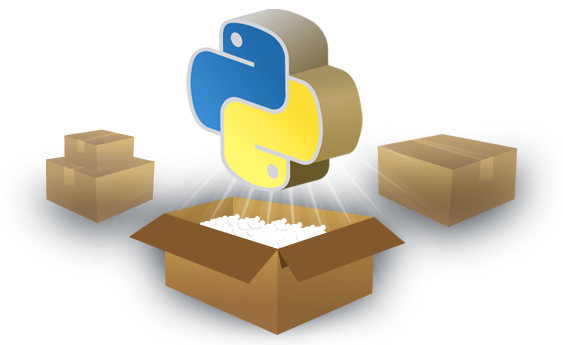
\includegraphics[width=6cm,height=3.68cm]{landing-about.png}
        %\caption{}
        \end{figure}
      \end{column}

      \end{columns}
      
    \end{frame}

    \begin{frame}{Python 2 vs. Python 3}
      \begin{columns}
      \begin{column}[t]{0.5\textwidth}
        Python 2.7.x
        \begin{itemize}
          \item print "hello world!"
          \item 3 / 2 \# 1
          \item 3 // 2 \# 1
          \item 3 / 2.0 \# 1.5
          \item 3 // 2.0 \# 1.0
        \end{itemize}
      \end{column}

      \begin{column}[t]{0.5\textwidth}
        Python 3.x
        \begin{itemize}
          \item print("hello world!")
          \item 3 / 2 \# 1.5
          \item 3 // 2 \# 1
          \item 3 / 2.0 \# 1.5
          \item 3 // 2.0 \# 1.0
        \end{itemize}
      \end{column}

      \end{columns}
      More differences: http://sebastianraschka.com/Articles/2014\_python\_2\_3\_key\_diff.html
      
    \end{frame}

    \begin{frame}{python 3的安装}
      
      官网: https://www.python.org \\
      文件下载: https://www.python.org/downloads/release/python-363/

      \begin{figure}
      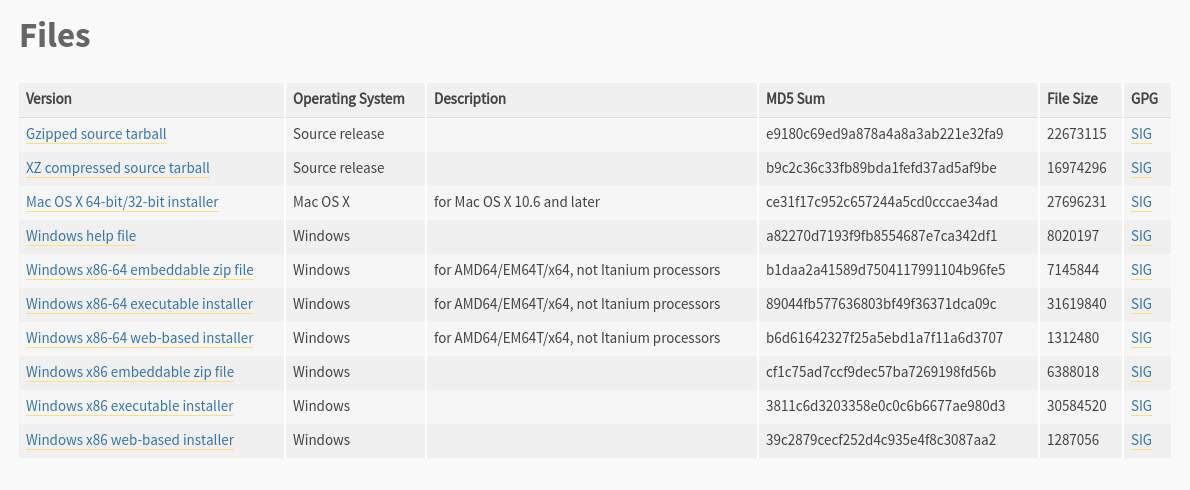
\includegraphics[height=5.35cm, width=13cm]{install-python.png}
      \caption{安装文件}
      \end{figure}
    \end{frame}

    \begin{frame}{Python vs. C/C++}
      \begin{columns}
      \begin{column}[t]{0.5\textwidth}
        \begin{figure}
        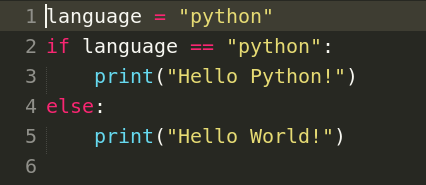
\includegraphics[height=2.17cm, width=5cm]{python-hello.png}
        \caption{python语法} 
        \end{figure}
        
      \end{column}

      \begin{column}[t]{0.5\textwidth}
        \begin{figure}
        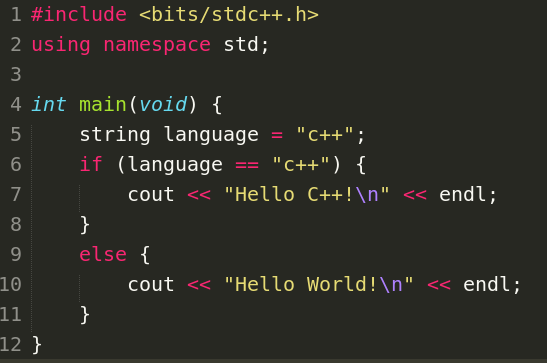
\includegraphics[height=3.98cm, width=6cm]{hello-c++.png}
        \caption{C/C++语法} 
        \end{figure}
        
      \end{column}

      \end{columns}
      
      
    \end{frame}

    

    \begin{frame}{variable 变量}
      \begin{itemize}
        \item num = 123
        \item string = 'abc'
        \item tp = (1,2,3)
        \item li = [1,2,3]
        \item chars = \{'a', 'b', 'c', 'd'\}
        \item dic = \{'height':10, 'width':20\}
      \end{itemize}
      
    \end{frame}

    \begin{frame}{type 类型}
      \begin{itemize}
        \item type(num) \# int
        \item type(string) \# str
        \item type(tp) \# tuple
        \item type(li) \# list
        \item type(chars) \# set
        \item type(dic) \# dict
      \end{itemize}
      
    \end{frame}

    \begin{frame}{list}
      \begin{itemize}
        \item li = []
        \item li = [1,2,3]
        \item li = ['l','o','v','e']
        \item li = [1,'love',3]
        \item li = list()
        \item li = list((1,'love',3))
      \end{itemize}
      
    \end{frame}

    

\end{document}

